\section{Performance Degradation} \label{sec:performance-degradation}

\begin{frame}{Performance Degradation}
    
    The performance of a model can be severely affected by dataset shift due to the model's inability to generalise to the new data distribution.
    
    We explored the impact of dataset shift on the performance of different ensemble methods:
    
    \begin{itemize}
        \item \textbf{Random Forest}
        \item \textbf{Gradient Boosting}
        \item \textbf{XGBoost}
    \end{itemize}

    Moreover we used a simple \textbf{logistic regression} model as a baseline for comparison.

\end{frame}

\begin{frame}{Performance Metric}
    
    We used the \textbf{Area Under the Receiver Operating Characteristic Curve (AUC-ROC)} as the performance metric for our models.

    \begin{figure}
        \centering
        \vfill
        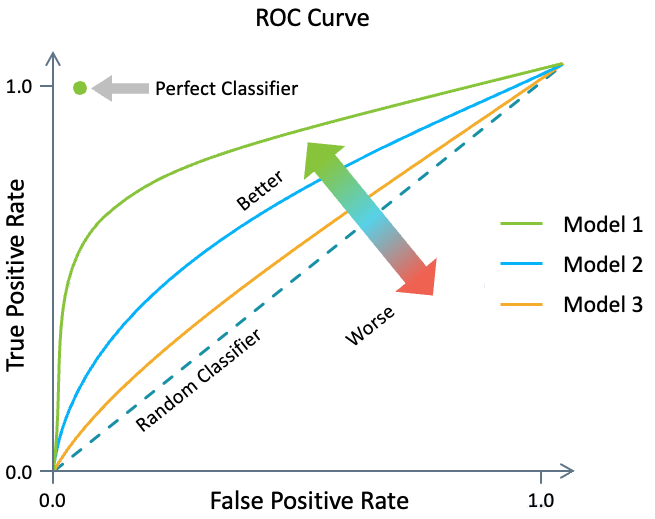
\includegraphics[width=0.6\textwidth]{roc_auc.png}
    \end{figure}

    The AUC-ROC ranges from 0 to 1, with a higher value indicating better performance.

\end{frame}

\begin{frame}{Fine Tuning}
    
    We performed a \textbf{hyperparameter tuning} to optimise the performance of our models. to do this, we used the \textbf{Grid Search} method with 5-fold cross-validation.

    \begin{figure}
        \centering
        \vfill
        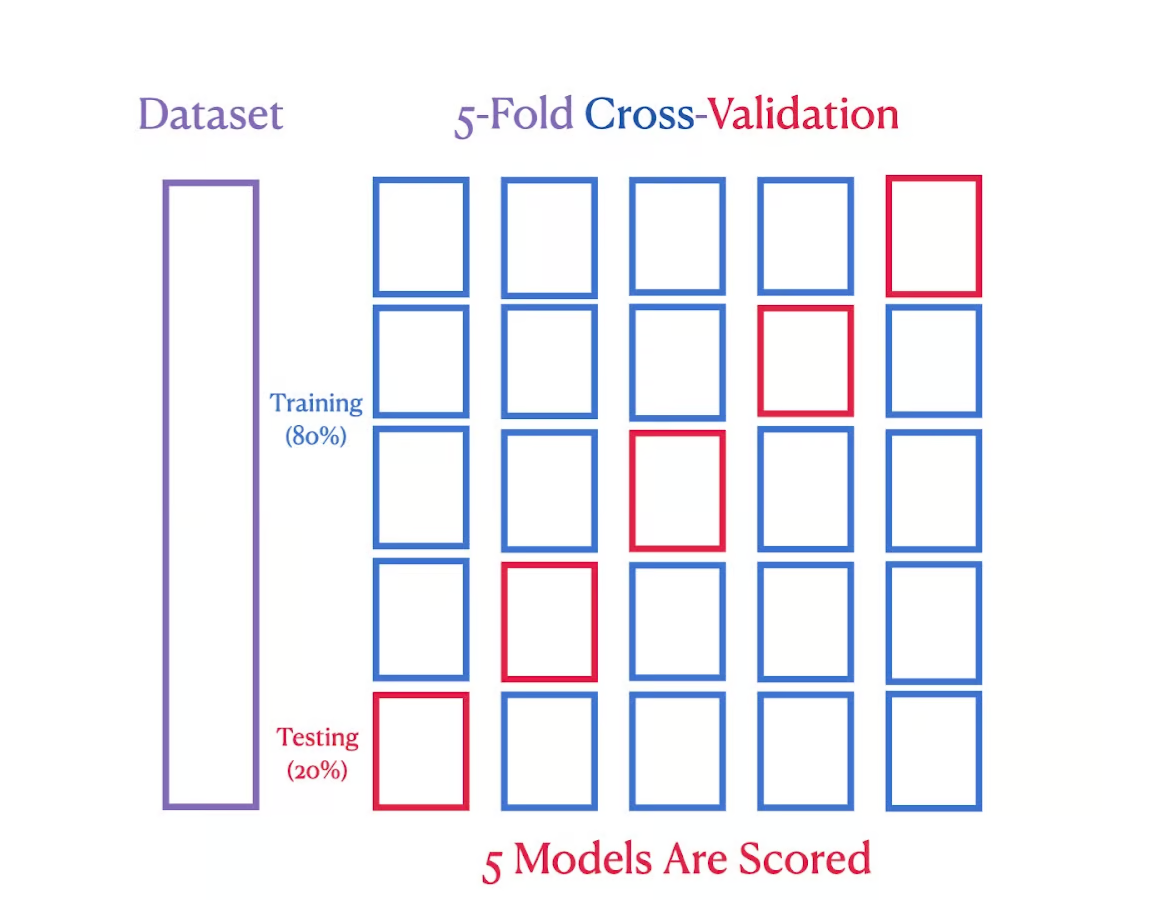
\includegraphics[width=0.6\textwidth]{k-fold.png}
    \end{figure}

\end{frame}

\begin{frame}{Logistic Regression}

    \textbf{Logistic Regression} is a simple linear model used for binary classification.

    $$
    \text{TODO}
    $$

\end{frame}

\begin{frame}{Random Forests}

    \textbf{Random Forest} is an ensemble learning method that builds multiple decision trees during training. 

    \begin{columns}
        \begin{column}{0.45\textwidth}
            It outputs the class that is the majority vote of the individual trees.

            \vspace{1em}

            {\small
            $$
            \begin{array}{|l|c|}
                \hline
                \textbf{Hyperparameter} & \textbf{Value} \\
                \hline
                \hline
                n\_estimators & 125 \\
                criterion & gini \\
                max\_depth & 5 \\
                min\_samples\_split & 5 \\
                min\_samples\_leaf & 1 \\
                \hline
            \end{array}
            $$
            }
        \end{column}
        \begin{column}{0.55\textwidth}
            \begin{figure}
                \centering
                \vfill
                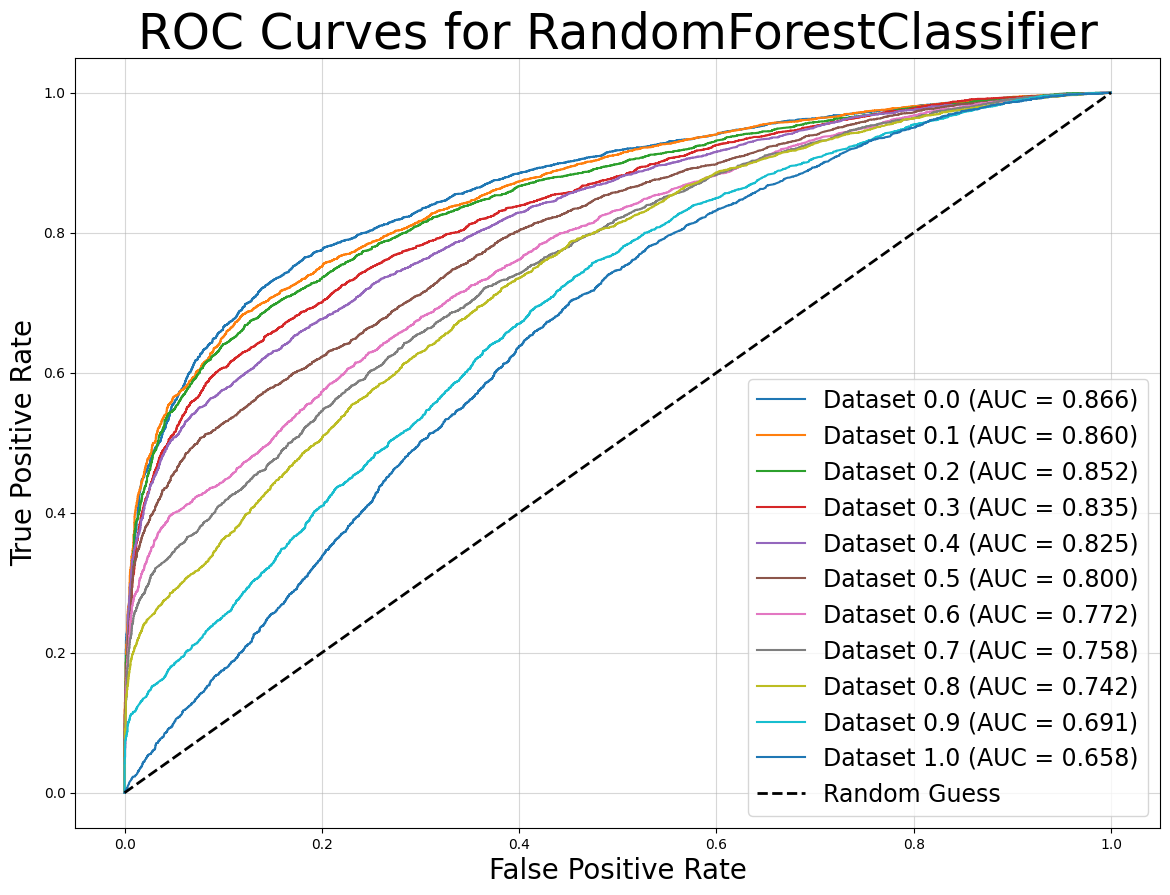
\includegraphics[width=\textwidth]{rf_auc.png}
            \end{figure}
        \end{column}
    \end{columns}

        \begin{footnotesize}
            \centering
            \textbf{Note:} We set \texttt{random\_state} to \texttt{0} for reproducibility.
        \end{footnotesize}
\end{frame}

\begin{frame}{Gradient Boosting}

    \textbf{Gradient Boosting} combines weak predictive models (usually decision trees) in an iterative manner.

    \begin{columns}
        \begin{column}{0.45\textwidth}
            Each model corrects the errors of its predecessor, making it highly effective but sensitive to hyperparameter tuning.

            \vspace{-0.1em}

            {\small
            $$
            \begin{array}{|l|c|}
                \hline
                \textbf{Hyperparameter} & \textbf{Values} \\
                \hline
                \hline
                n\_estimators & 125 \\
                learning\_rate & 0.025 \\
                max\_depth & 3 \\
                subsample & 0.4 \\
                \hline
            \end{array}
            $$
            }
        \end{column}
            \begin{column}{0.55\textwidth}
                \begin{figure}
                    \centering
                    \vfill
                    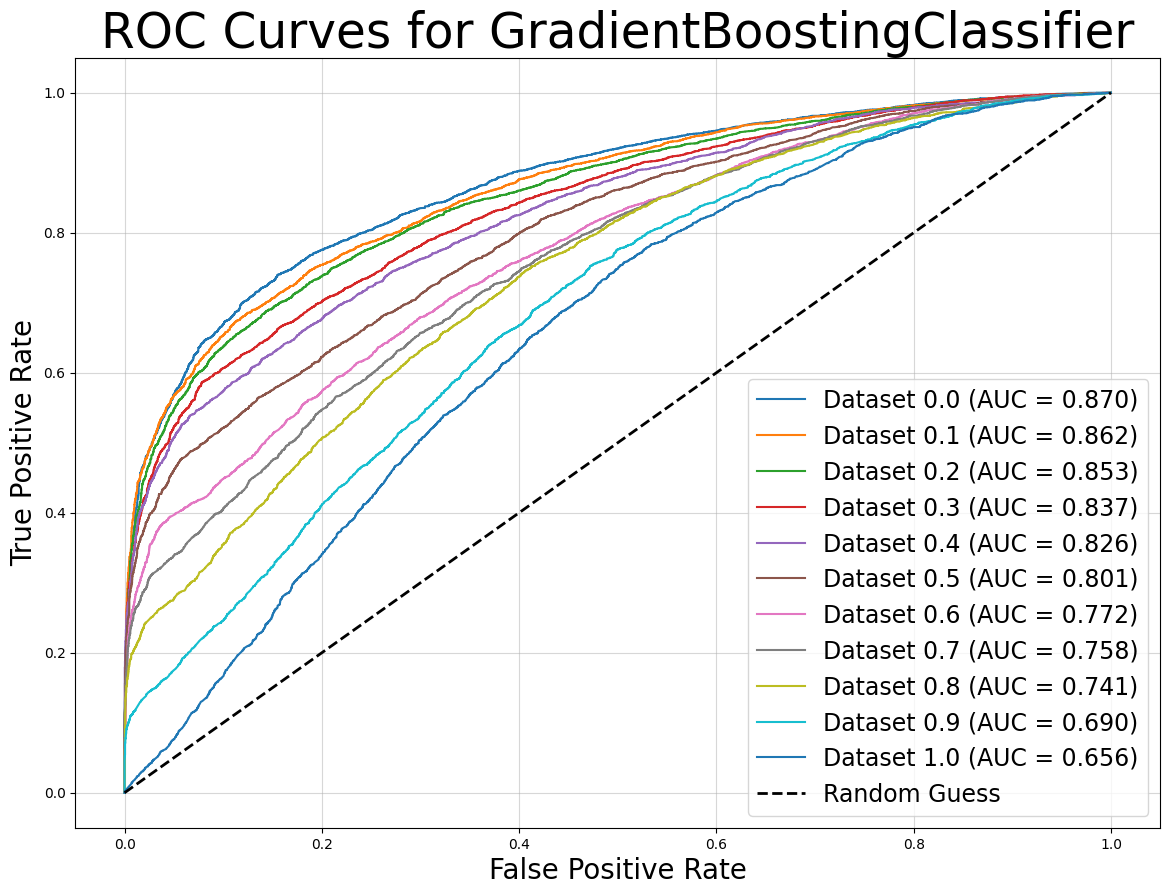
\includegraphics[width=\textwidth]{gbc_auc.png}
                \end{figure}
            \end{column}
    \end{columns}

\end{frame}

\begin{frame}{Extreme Gradient Boosting}

    \textbf{XGBoost} (\textit{Extreme Gradient Boosting}) is a scalable and efficient gradient boosting framework known for its regularization capabilities and speed.

    \begin{columns}
        \begin{column}{0.45\textwidth}
            {\small
            $$
            \begin{array}{|l|c|}
                \hline
                \textbf{Hyperparameter} & \textbf{Values} \\
                \hline
                \hline
                n\_estimators & 100 \\
                learning\_rate & 0.1 \\
                max\_depth & 6 \\
                subsample & 0.7 \\
                gamma & 5 \\
                \hline
            \end{array}
            $$
            }
        \end{column}
        \begin{column}{0.55\textwidth}
            \begin{figure}
                \centering
                \vfill
                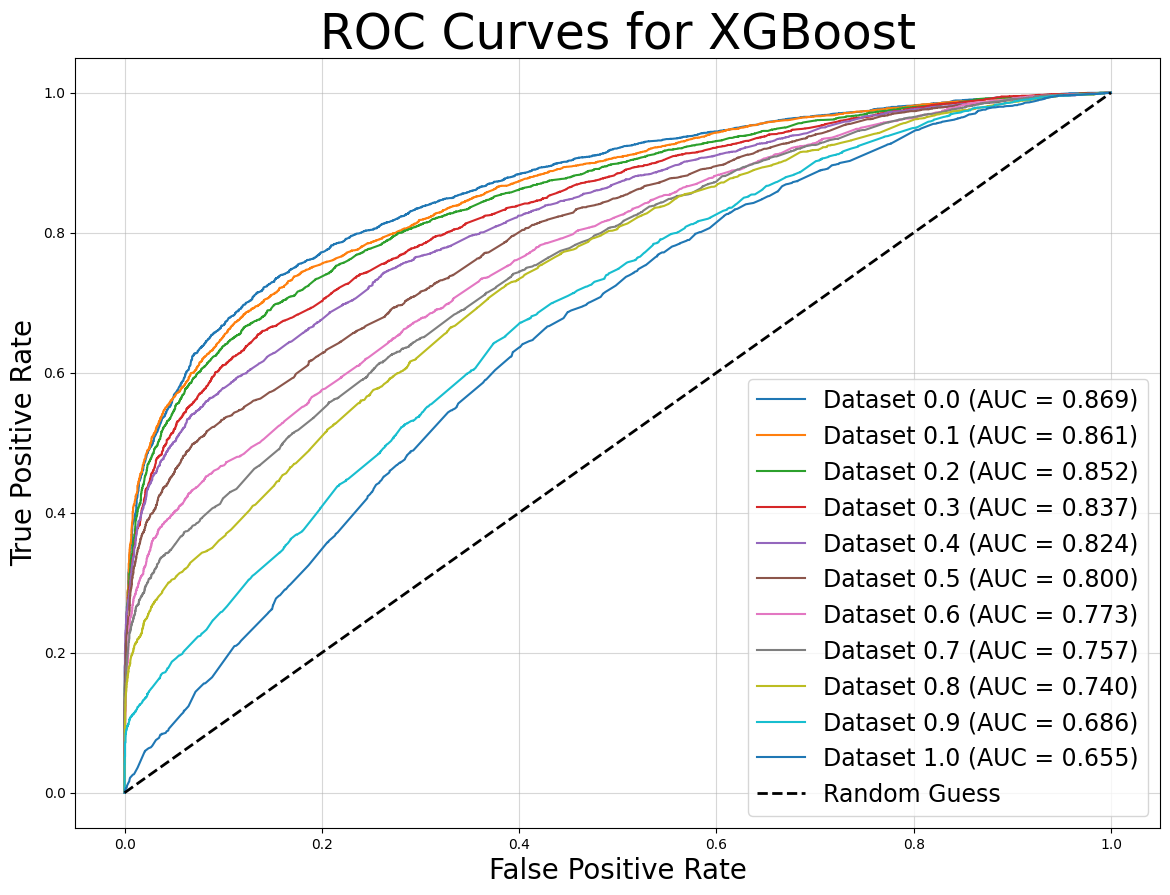
\includegraphics[width=\textwidth]{xgb_auc.png}
            \end{figure}
        \end{column}
    \end{columns}
\end{frame}

\begin{frame}{Performance Comparison}

    \begin{figure}
        \centering
        \vfill
        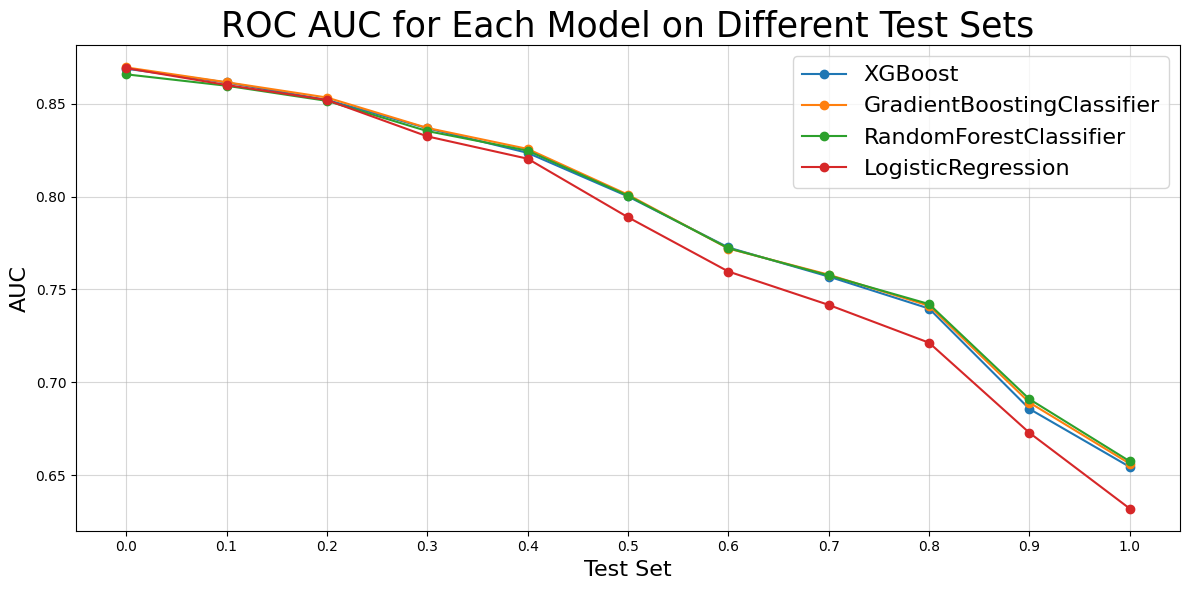
\includegraphics[width=\textwidth]{auc_comp.png}
    \end{figure}

\end{frame}

\begin{frame}{Performance Comparison}

    \begin{figure}
        \centering
        \vfill
        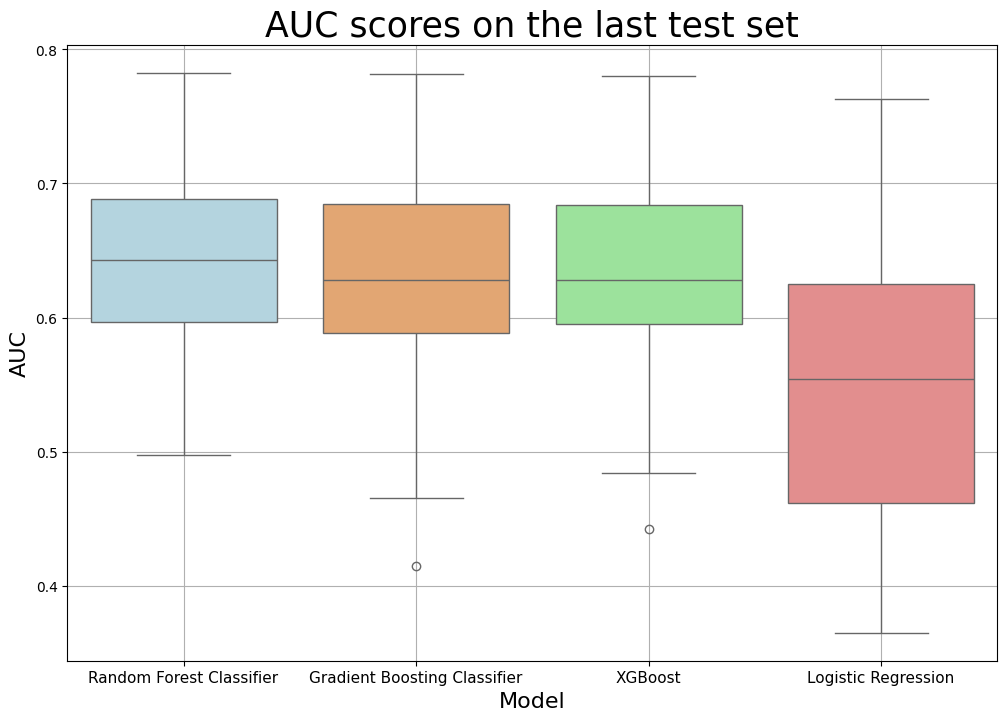
\includegraphics[width=0.8\textwidth]{boxplot.png}
    \end{figure}

\end{frame}
